\chapter{Linear Systems}
\label{chap:linear-systems}

Linear systems are by definition sets of linear equations, that is, of equations
which relate present variables in a \emph{linear} way. It is important to
understand what this means. Spelled out, an expression on either side of any of
the equations is formed \emph{solely} by
\begin{enumerate}
 \item multiplying the variables by a given number (\textbf{not another
  variable}),
 \item adding these multiples together.
\end{enumerate}
Any such combination where variables are only allowed to be multiplied by a
constant and added is called a \emph{linear combination}. This term is extremely
important and ubiquitous throughout the text; hence, it warrants an isolated
definition. 

\begin{definition}{Linear combination}{linear-combination}
 Let $x_1,\ldots,x_n$ with $n \in \N$ be variables. Their \emph{linear
 combination} is any expression of the form
 \[
  a_1x_1 + a_2x_2 + \cdots + a_n x_n,
 \]
 where $a_1,\ldots,a_n$ are numbers.
\end{definition}

\begin{remark}{}{linear-combination}
 In the \hyperref[def:linear-combination]{definition above}, we have
 deliberately not specified what type of \emph{numbers} we mean. In the future,
 we shall work extensively with real and complex numbers as well as elements of
 other fields, which dear readers might not have even recognised as `numbers'
 thus far. The only important concept in this regard is the clear distinction
 between a \emph{number} (later \emph{scalar}) and a \emph{variable} (later
 \emph{vector}).
\end{remark}

\begin{example}{}{linear-combination}
 Consider the variables $x,y$ and $z$. The expression
 \[
  3x + 2y - 0.5z
 \]
 \textbf{is} their linear combination whereas
 \[
  5x + 3y - yz + 7z^2
 \]
 \textbf{is not}.
\end{example}

To reiterate, a \emph{linear system} is any set of equations featuring only
linear combinations of variables; these equations are consequently called
\emph{linear} as well. A \emph{solution} of a linear system is the set of all
possible substitutions of numbers (in place of variables) which make the
equations true.

It is clear that every linear equation can be rearranged to
\[
 a_1 x_1 + \cdots + a_n x_n = c
\]
for some variables $x_1,\ldots,x_n$ and numbers $a_1,\ldots,a_n,c$ by simple
subtraction. This is how we shall define it, for simplicity.

\begin{definition}{Linear equation}{linear-equation}
 Any equation of the form
 \begin{equation}
  \label{eq:linear-equation}
  a_1x_1 + a_2x_2 + \cdots + a_n x_n = c,
 \end{equation}
 where $x_1,\ldots,x_n$ are variables and $a_1,\ldots,a_n,c$ are numbers, is
 called \emph{linear}. A \emph{solution} of a linear equation is an $n$-tuple
 $(b_1,\ldots,b_n)$ of numbers such that under the substitutions $x_i \coloneqq
 b_i$, for $i \in \{1,\ldots,n\}$, the equation~\eqref{eq:linear-equation} is
 satisfied.
\end{definition}

\begin{example}{}{linear-equation}
 The equation
 \[
  3x_1 - 2x_2 + 4x_3 + x_4 = 5
 \]
 is \hyperref[def:linear-equation]{linear} in variables $x_1,x_2,x_3$ and $x_4$.
 On the contrary,
 \[
  3x_1x_2 - 4x_3^2 = 10
 \]
 is \textbf{not} linear.
\end{example}

\begin{definition}{Linear system}{linear-system}
 Any set of linear equations in the given variables $x_1,\ldots,x_n$ is called a
 \emph{linear system}. A \emph{solution} of a linear system is an $n$-tuple
 $(b_1,\ldots,b_n)$ which solves every linear equation in the set.
\end{definition}

\begin{example}{}{linear-system}
 The set of equations
 \[
  \begin{array}{rcrcrcr}
   3x_1 & - & x_2 & + & 2x_3 &= &1\\
   x_1 & & & - & x_3 &= &-1 \\
   2x_1 & - & 3x_2 & + & 3x_3 & = & 0
  \end{array}
 \]
 is a \hyperref[def:linear-system]{linear system} whose solution is the triple
 $(0,1,1)$.
\end{example}

%TODO reference
We proceed to discuss two trivial examples, which readers might have discussed
in high school, naturally leading to linear systems. More sophisticated examples
are presented in the applications section.

\begin{example}{Static equations}{static-equations}
 Suppose we have three objects -- one with a mass of $2$ and the other two with
 masses unknown. Experimentation produces these two balances.
 \begin{figure}[H]
  \centering
  \begin{subfigure}[b]{.45\textwidth}
   \centering
   \begin{tikzpicture}
    \node[isosceles triangle, draw, fill=black!30, anchor=left corner, shape
     border rotate=90, minimum height=5mm, minimum width=1cm, isosceles
     triangle stretches] (base) at (0,0) {};
    \coordinate[left=3 of base.north] (left);
    \coordinate[right=3 of base.north] (right);
    \draw (left) -- (right);

    \node[circle,draw,left=0.75cm of base.north,minimum height=6mm,inner
     sep=0,yshift=3mm] (x) {$x$};
    \node[circle,draw,left=2cm of base.north,minimum height=4mm,inner
     sep=0,yshift=2mm] (y) {$y$};
    \node[circle,draw,right=2.5cm of base.north,minimum height=5mm,inner
     sep=0,yshift=2.5mm] (two) {$2$};

    \coordinate[above=2cm of base.north] (above);
    \draw[dashed] (base.north) -- (above);
    \draw[dashed] (x.north) -- ($(above) - (1.05,0)$);
    \draw[dashed] (y.north) -- ($(above) - (2.2,0)$);
    \draw[dashed] (two.north) -- ($(above) + (2.75,0)$);

    \draw[<->,thick] ($(x.north) + (0,0.5)$) to
     node[midway,circle,fill=white,inner sep=1pt] {$15$} ($(x.north) +
     (1.05,0.5)$);
    \draw[<->,thick] ($(y.north) + (0,1.25)$) to
     node[midway,circle,fill=white,inner sep=1pt] {$40$} ($(y.north) +
     (2.2,1.25)$);
    \draw[<->,thick] ($(two.north) + (0,1.15)$) to
     node[midway,circle,fill=white,inner sep=1pt] {$50$} ($(two.north) +
     (-2.75,1.15)$);
   \end{tikzpicture}
  \end{subfigure}
  \hspace*{\fill}
  \begin{subfigure}[b]{.45\textwidth}
   \centering
   \begin{tikzpicture}
    \node[isosceles triangle, draw, fill=black!30, anchor=left corner, shape
     border rotate=90, minimum height=5mm, minimum width=1cm, isosceles
     triangle stretches] (base) at (0,0) {};
    \coordinate[left=3 of base.north] (left);
    \coordinate[right=3 of base.north] (right);
    \draw (left) -- (right);

    \node[circle,draw,left=1.25cm of base.north,minimum height=6mm,inner
     sep=0,yshift=3mm] (x) {$x$};
    \node[circle,draw,right=2.5cm of base.north,minimum height=4mm,inner
     sep=0,yshift=2mm] (y) {$y$};
    \node[circle,draw,right=1.25cm of base.north,minimum height=5mm,inner
     sep=0,yshift=2.5mm] (two) {$2$};

    \coordinate[above=2cm of base.north] (above);
    \draw[dashed] (base.north) -- (above);
    \draw[dashed] (x.north) -- ($(above) - (1.55,0)$);
    \draw[dashed] (y.north) -- ($(above) + (2.7,0)$);
    \draw[dashed] (two.north) -- ($(above) + (1.5,0)$);

    \draw[<->,thick] ($(x.north) + (0,1.05)$) to
     node[midway,circle,fill=white,inner sep=1pt] {$25$} ($(x.north) +
     (1.55,1.05)$);
    \draw[<->,thick] ($(y.north) + (0,1.25)$) to
     node[midway,circle,fill=white,inner sep=1pt] {$50$} ($(y.north) +
     (-2.7,1.25)$);
    \draw[<->,thick] ($(two.north) + (0,0.6)$) to
     node[midway,circle,fill=white,inner sep=1pt] {$25$} ($(two.north) +
     (-1.5,0.6)$);
   \end{tikzpicture}
  \end{subfigure}
 \end{figure}

 For the weights to be in balance, the sums of \emph{moments} on both sides of
 the scales must be identical one to another. A \emph{moment} of an object is
 its distance from the centre of the scales times its mass. This condition
 yields a system of two linear equations
 \[
  \begin{array}{ccccccc}
   15x & + & 40y & = & 50 \cdot 2, & &\\
       &   & 25x & = & 25 \cdot 2 & + & 50y.
  \end{array}
 \]
 Or, after rearrangement (to stay true to \hyperref[def:linear-equation]{our
 definition of linear equation}),
 \[
  \begin{array}{ccccc}
   15x & + & 40y & = & 50 \cdot 2,\\
   25x & - & 50y & = & 25 \cdot 2.
  \end{array}
 \]
\end{example}

\begin{example}{Chemical reactions}{chemical-reactions}
 Toluene, $\mathtt{C_7 H_8}$, mixes (under right conditions) with nitric acid,
 $\mathtt{HNO_3}$, to produce trinitrotoluene (widely known as TNT),
 $\mathtt{C_7H_5O_6N_3}$, along with dihydrogen monoxide, $\mathtt{H_2O}$. If we
 want this chemical reaction to occur successfully, we must (among other things)
 ascertain we mix the constituents in the right proportion. In pseudo-chemical
 notation, the reaction to take place can be written as
 \[
  x \cdot \mathtt{C_7H_8} + y \cdot \mathtt{HNO_3} \longrightarrow z \cdot
  \mathtt{C_7H_5O_6N_3} + w \cdot \mathtt{H_2O}.
 \]
 Comparing the number of atoms of each element before the reaction and
 afterwards (which must remain identical owing to the conservation of energy)
 yields the system
 \[
  \begin{array}{cccccccc}
   \mathtt{H}: & 8x & + & 1y & = & 5z & + & 2w,\\
   \mathtt{C}: & 7x &   &    & = & 7z,&   &\\
   \mathtt{N}: &    &   & 1y & = & 3z,&   &\\
   \mathtt{O}: &    &   & 3y & = & 6z & + & 1w.
  \end{array}
 \]
\end{example}

In the next section, we devise an algorithm to solve any system of linear
equations.

\section{Gauss-Jordan Elimination}
\label{sec:gauss-jordan-elimination}

Probably the most well-known algorithm for solving a
\hyperref[def:linear-system]{linear system} is the \emph{Gauss-Jordan
Elimination}. As its name partially implies, its heart lies in the
\emph{elimination} of variables one by one, until only a single linear equation
in one variable stands unsolved. This is done by applying different
\emph{transformations} to the initial system that are guaranteed not to alter
the solution. We're going to solve a linear system first and describe the
general method second.

\begin{problem}{}{gauss-jordan-elimination}
 Solve the linear system
 \[
  \begin{array}{rcrcrcr}
   & & & & 3x_3 & = & 9\\
   x_1 & + & 5x_2 & - & 2x_3 & = & 2\\
   \frac{1}{3}x_1 & + & 2x_2 & & & = & 3
  \end{array}.
 \]
\end{problem}
\begin{probsol}
 We aim to transform the system step by step to a form which allows us to
 (successively) eliminate all variables.

 The first transformation entails a simple exchange of the first and third row.
 \begin{center}
  \begin{tikzpicture}
   \node (eq) at (0,0) {$
     \begin{array}{rcrcrcr}
      \frac{1}{3}x_1 & + & 2x_2 & & & = & 3\\
      x_1 & + & 5x_2 & - & 2x_3 & = & 2\\
      & & & & 3x_3 & = & 9
     \end{array}.
   $};
  \coordinate (eqsw) at ($(eq.south west) + (-0.2,0.36)$);
  \coordinate (eqnw) at ($(eq.north west) - (0.2,0.36)$);
  \draw[<->,thick] (eqsw) to[bend left=90,looseness=2] (eqnw);
  \node at (-4.9,0) {\footnotesize \texttt{Swapped first and third row.}};
  \end{tikzpicture}
 \end{center}
 Next, we shall scale the first row by a factor of $3$.
 \begin{center}
  \begin{tikzpicture}
   \node (eq) at (0,0) {$
     \begin{array}{rcrcrcr}
      x_1 & + & 6x_2 & & & = & 9\\
      x_1 & + & 5x_2 & - & 2x_3 & = & 2\\
      & & & & 3x_3 & = & 9
     \end{array}.
   $};
  \coordinate (eqnw) at ($(eq.north west) - (0.2,0.36)$);
  \coordinate (start) at ($(eqnw) - (1,0)$);
  \draw[->,thick] (start) to node[midway,yshift=2mm] {\footnotesize
   $\mathtt{\cdot 3}$} (eqnw);
  \node at ($(start) - (2,0)$) {\footnotesize \texttt{Scaled the first row by
   3.}};
  \end{tikzpicture}
 \end{center}
 Finally, we subtract the first row from the second row. Said in a more
 foreshadowing manner, we add the $(-1)$-multiple of the first row to the second
 row.
 \begin{center}
  \begin{tikzpicture}
   \node (eq) at (0,0) {$
     \begin{array}{rcrcrcr}
      x_1 & + & 6x_2 & & & = & 9\\
       & - & x_2 & - & 2x_3 & = & -7\\
      & & & & 3x_3 & = & 9
     \end{array}.
   $};
  \coordinate (row1) at ($(eq.north west) - (0.2,0.36)$);
  \coordinate (row2) at ($(eq.west) - (0.2,0)$);
  \draw[->,thick] (row1) to[bend right=90,looseness=2] node[midway,xshift=-4mm]
   (mid) {\footnotesize $\mathtt{\cdot (-1)}$} (row2);
  \node at ($(mid) - (3.5,0)$) {\footnotesize \texttt{Subtracted the first row
   from the second.}};
  \end{tikzpicture}
 \end{center}
 These transformations have wrought the system into a state where it can be
 easily solved.

 Indeed, we immediately see that the third equation implies $x_3 = 3$.
 Substituting into the second equation gives 
 \[
  -x_2 - 2 \cdot 3 = -7
 \]
 whose solution is $x_2 = 1$. Finally, knowing the value of $x_2$, we can solve
 the first equation by another substitution. We get
 \[
  x_1 + 6 \cdot 1 = 9,
 \]
 thus $x_1 = 3$ and the triple $(3,1,3)$ is the \emph{unique} solution of the
 system.
\end{probsol}

Observant readers might have already identified the `kinds' of transformations
that were used in solving the \hyperref[prob:gauss-jordan-elimination]{linear
system above}. Nonetheless, we're about to spell them out.

The transformations that do not change the solution of a
\hyperref[def:linear-system]{linear system} include
\begin{enumerate}
 \item swapping two equations;
 \item scaling an equation by a non-zero constant;
 \item adding a multiple of an equation to \emph{another} equation.
\end{enumerate}
Note that transformations (2) and (3) come with sensible restrictions. Scaling
an equation by $0$ clearly changes the set of solutions of the system as it
basically removes the equation entirely. Adding a multiple of an equation to
\emph{itself} suffers from the same problem; it might result in `invalidating'
the equation should the scaling factor be $-1$.

We know proceed to prove that transformations (1) - (3) truly do not alter the
solutions of the initial system.

\begin{theorem}{Gauss-Jordan}{gauss-jordan}
 The transformations (1) - (3) of a linear system outlined above do not change
 its solution set.
\end{theorem}
\begin{thmproof}
 We will cover transformation (3) here. The proofs for transformations (1) and
 (2) are similar and thus left as an exercise.

 Consider the linear system
 \[
  \begin{array}{rcrcccrcr}
   a_{1,1}x_1 & + & a_{1,2}x_2 & + & \cdots & + & a_{1,n}x_n & = & c_1\\
   a_{2,1}x_1 & + & a_{2,2}x_2 & + & \cdots & + & a_{2,n}x_n & = & c_2\\
              &   &            &   &        &   &            & \vdots &\\
   a_{m,1}x_1 & + & a_{m,2}x_2 & + & \cdots & + & a_{m,n}x_n & = & c_m
  \end{array}
 \]
 of $m$ equations in variables $x_1,\ldots,x_n$ and let $(b_1,\ldots,b_n)$ be
 one of its solutions. Choose a constant $k$ and add the $k$-multiple of the
 $i$-th equation to the $j$-th equations for some $i,j \in \{1,\ldots,m\}$.
 Hence, the $j$-th equation of the system gets replaced by
 \[
  (a_{j,1} + k \cdot a_{i,1})x_1 + (a_{j,2} + k \cdot a_{i,2})x_2 + \cdots +
  (a_{j,n} + k \cdot a_{i,n})x_n = c_j + k \cdot c_i,
 \]
 which can be rearranged to
 \begin{equation}
  \label{eq:gauss-jordan}
  a_{j,1}x_1 + a_{j,2}x_2 + \cdots + a_{j,n}x_n + k \cdot (a_{i,1}x_1 +
  a_{i,2}x_2 + \cdots + a_{i,n}x_n) = c_j + k \cdot c_i.
 \end{equation}
 Since $(b_1,\ldots,b_n)$ is a solution of the original system, we know that
 \[
  \begin{array}{rcrcccrcr}
   a_{i,1}b_1 & + & a_{i,2}b_2 & + & \cdots & + & a_{i,n}b_n & = & c_i\\
   a_{j,1}b_1 & + & a_{j,2}b_2 & + & \cdots & + & a_{j,n}x_n & = & c_j
  \end{array}.
 \]
 Substituting this into equation~\eqref{eq:gauss-jordan} gives
 \[
  c_j + k \cdot c_i = c_j + k \cdot c_i,
 \]
 hence $(b_1,\ldots,b_n)$ is also the solution of the transformed system, as
 required.
\end{thmproof}

\begin{exercise}{}{gauss-jordan}
 Show that transformations (1) and (2) also don't change the set of solutions of
 the transformed linear system.
\end{exercise}

\begin{definition}{Elementary operations}{elementary-operations}
 The transformations (1) - (3) outlined above are called \emph{elementary
 operations} or \emph{row operations}.
\end{definition}

As we've seen in \myref{problem}{prob:gauss-jordan-elimination}, the application
of transformations (1) - (3) has its purpose in preparing the system for a final
back-substitution, where the values of all variables in a row save the first one
are known beforehand. A system which is `ready' to be solved by
back-substitution is said to be in \emph{echelon form}.

\begin{definition}{Echelon form}{echelon-form}
 In each row of a \hyperref[def:linear-system]{linear system}, the first
 variable with a non-zero coefficient is called the row's \emph{leading
 variable}.

 A linear system is in \emph{echelon form} (or \emph{upper triangular form}) if
 the leading variable in each row is at least one column to the right of the
 leading variable in the row above and all rows filled with zeroes are at the
 bottom.
\end{definition}

\begin{example}{}{echelon-form}
 The system
 \[
  \begin{array}{rcrcrcr}
   x_1 & + & 6x_2 & & & = & 9\\
    & - & x_2 & - & 2x_3 & = & -7\\
   & & & & 3x_3 & = & 9
  \end{array}
 \]
 \textbf{is} in echelon form whereas
 \[
  \begin{array}{rcrcrcr}
   2x_1 & + & 3x_2 & - & x_3 & = & 9\\
    & & 3x_2 & - & 2x_3 & = & 2\\
    x_1 & & & - & x_3 & = & 0
  \end{array}
 \]
 is \textbf{not}.
\end{example}

For now, we shall employ intuition and a nibble of foresight to guide our
transformation of a \hyperref[def:linear-system]{linear system} into its
\hyperref[def:echelon-form]{echelon form}. Later, we intend to present a precise
algorithm (that computers also use) that achieves this.

\begin{example}{}{echelon-form-2}
 We're going to put the system
 \[
  \begin{array}{rcrcrcr}
    x_1 & + & x_2 & & & = & 0\\
    2x_1 & - & x_2 & + & 3x_3 & = & 3\\
    x_1 & - & 2x_2 & - & x_3 & = & 3
  \end{array}
 \]
 into echelon form and solve it using back-substitution. We'll label the rows of
 the system by Roman letters and denote transformations accordingly. For
 example, adding a $3$-multiple of row one to row three would be written
 symbolically as $\mathtt{3 \cdot I + III}$.

 First, we need to get rid of the variable $x_1$ in rows \texttt{II} and
 \texttt{III}. This can be done by subtracting adequate multiples of row
 \texttt{I}.
 \begin{center}
  \begin{tikzpicture}
   \node at (-6,0) {$
    \begin{array}{rcrcrcr}
      x_1 & + & x_2 & & & = & 0\\
      2x_1 & - & x_2 & + & 3x_3 & = & 3\\
      x_1 & - & 2x_2 & - & x_3 & = & 3
    \end{array}
    $};
   \node (eq) at (0,0) {$
    \begin{array}{rcrcrcr}
      x_1 & + & x_2 & & & = & 0\\
      & - & 3x_2 & + & 3x_3 & = & 3\\
      & - & 3x_2 & - & x_3 & = & 3
    \end{array}
   $};
  \draw[|->,thick,shorten <=5pt, shorten >=5pt] ($(eq.west) - (2.5,0)$) to
   node[midway,yshift=2mm] {\footnotesize $\mathtt{-2I + II}$}
   node[midway,yshift=-2mm] {\footnotesize $\mathtt{-I + III}$} (eq.west);
  \end{tikzpicture}
 \end{center}
 We continue by subtracting row \texttt{II} from row \texttt{III}.
 \begin{center}
  \begin{tikzpicture}
   \node at (-6,0) {$
    \begin{array}{rcrcrcr}
      x_1 & + & x_2 & & & = & 0\\
      & - & 3x_2 & + & 3x_3 & = & 3\\
      & - & 3x_2 & - & x_3 & = & 3
    \end{array}
    $};
   \node (eq) at (0,0) {$
    \begin{array}{rcrcrcr}
      x_1 & + & x_2 & & & = & 0\\
      & - & 3x_2 & + & 3x_3 & = & 3\\
      & & & - & 4x_3 & = & 0
    \end{array}
   $};
  \draw[|->,thick,shorten <=5pt, shorten >=5pt] ($(eq.west) - (2.5,0)$) to
   node[midway,yshift=2mm] {\footnotesize $\mathtt{-II + III}$} (eq.west);
  \end{tikzpicture}
 \end{center}
 The system is now in \hyperref[def:echelon-form]{echelon form}. The equation in
 row \texttt{III} forces $x_3 = 0$. Substitution into row \texttt{II}
 immediately gives $x_2 = -1$ and one final substitution into row \texttt{I}
 yields $x_1 = 1$.

 Hence, the solution of the system is the triple $(1, -1, 0)$.
\end{example}

\begin{exercise}{}{echelon-form}
 Using \emph{Gauss-Jordan elimination} solve the systems from
 examples~\ref{exam:static-equations} and~\ref{exam:chemical-reactions}.
\end{exercise}

All the systems we've studied so far have had the same number of equations as
variables. This of course need not be the case in general. Thankfully,
Gauss-Jordan elimination can \emph{always} be used to determine the solution set
of a \hyperref[def:linear-system]{linear system}. However, this set can also be
empty or infinite in cases where the number of variables doesn't match the
number of equations. The following two examples illustrate this.

\begin{example}{}{echelon-form-3}
 The following system has more equations than variables.
 \begin{equation}
  \label{eq:overdetermined-system}
  \begin{array}{rcrcr}
    x_1 & + & 3x_2 & = & 1\\
    2x_1 & + & x_2 & = & -3\\
    2x_1 & + & 2x_2 & = & -2
  \end{array}
 \end{equation}
 Before we put it into \hyperref[def:echelon-form]{echelon form} and solve it,
 let us ponder what the solution set may look like. Intuitively, a linear
 equation is basically a `restraint' or `condition' on the range of possible
 values the present variables may attain. If there are three equations
 restraining only two variables, then this restraint may be too harsh and lead
 to the system having no solution at all. The only case where solution
 \emph{does} exist involves one of the equations being \emph{redundant} --
 providing no additional condition. Algebraically, this happens if said equation
 is a \hyperref[def:linear-combination]{linear combination} of the other two.

 To draw a `real-life' simile, imagine the price of an apple being \$5/kg and
 that of bananas \$1.5/kg. Saying that 3 kg of apples and 4 kg of bananas cost,
 say, \$30 is simply false because we can calculate that this amount actually
 costs \$21. The third condition on the price of apples and bananas contradicted
 the previous two; just as a third equation in a
 \hyperref[def:linear-system]{linear system} in two variables can contradict the
 first two equations. We tend to call such systems \emph{overdetermined} and
 will in time dedicate a section to finding a `good' approximation of their
 solution.

 To solve the system~\eqref{eq:overdetermined-system}, we transform it into
 echelon form. First, we subtract twice the first row from the other two.
 \begin{center}
  \begin{tikzpicture}
   \node at (-5.5,0) {$
    \begin{array}{rcrcr}
      x_1 & + & 3x_2 & = & 1\\
      2x_1 & + & x_2 & = & -3\\
      2x_1 & + & 2x_2 & = & -2
    \end{array}
   $};
   \node (eq) at (0,0) {$
    \begin{array}{rcrcr}
      x_1 & + & 3x_2 & = & 1\\
      & & -5x_2 & = & -5\\
      & & -4x_2 & = & -4
    \end{array}
   $};
  \draw[|->,thick,shorten <=5pt, shorten >=5pt] ($(eq.west) - (2.5,0)$) to
   node[midway,yshift=2mm] {\footnotesize $\mathtt{-2I + II}$}
   node[midway,yshift=-2mm] {\footnotesize $\mathtt{-2I + III}$}(eq.west);
  \end{tikzpicture}
 \end{center}
 Finally, we add $(-4 / 5)$-times row \texttt{II} to row \texttt{III}.
 \begin{center}
  \begin{tikzpicture}
   \node at (-6,0) {$
    \begin{array}{rcrcr}
      x_1 & + & 3x_2 & = & 1\\
      & & -5x_2 & = & -5\\
      & & -4x_2 & = & -4
    \end{array}
   $};
   \node (eq) at (0,0) {$
    \begin{array}{rcrcr}
      x_1 & + & 3x_2 & = & 1\\
      & & -5x_2 & = & -5\\
      & & 0 & = & 0
    \end{array}
   $};
  \draw[|->,thick,shorten <=5pt, shorten >=5pt] ($(eq.west) - (3,0)$) to
   node[midway,yshift=2mm] {\footnotesize $\mathtt{-(4 / 5)II + III}$}
   (eq.west);
  \end{tikzpicture}
 \end{center}
 Clearly, the third equation is \emph{redundant} because it provides no
 condition on the values of the variables. Back-substitution yields $x_2 = 1$
 and $x_1 = -2$. As we've claimed (but not yet proven), row \texttt{III} is
 indeed a linear combination of rows \texttt{I} and \texttt{II}. In this
 particular case, it holds that $\mathtt{(2 / 5)I + (4 / 5)II = III}$.
\end{example}

\section{Visualizing Linear Systems}
\label{sec:visualizing-linear-systems}

In this, rather informal, section, we present a way to visualize linear systems
in two and three variables and their solutions. Why two and three, you ask? The
number of variables in a linear equation determines the \emph{dimension} of the
\emph{geometric object} described by this equation. We shall soon provide the
necessary definitions to make rigorous sense of the sentence previous.
Intuitively, each variable represents a new `direction' we're allowed to move
in. Therefore, linear equations in two variables live in two-dimensional spaces
and linear equations in three variables occupy three dimensions.

Nonetheless, the equations themselves (if non-trivial) never describe objects of
the maximal possible dimension but of the dimension lower by one. This is
because they establish a relationship between the variables -- a relationship
where one variable grows entirely dependent on the rest, essentially `locking' a
single direction of movement. Think of it like this: a linear equation in two
variables is a sort of order, telling you that for every step forward you must
also make (say) two steps to the right, thereby rendering you unable to ever
walk in a direction different from the initial.

We proceed to show that the objects described by linear equations in two
variables are \emph{straight lines}. Said `objects described' are formally the
sets of points satisfying given equations. For instance, the object described by
the equation $3x + 2y = 4$ is the set
\[
 L \coloneqq \{(x,y) \in \R^2 \mid 3x + 2y = 4\}.
\]
Before we move on, we need establish an important fact. What is a \emph{straight
line} \textbf{exactly}? Wishing not to cheat and define straight line as the
object described by a linear equation, we employ a more geometric approach to
the definition. As we hope dear readers agree, a (one-dimensional) object is
\emph{straight} if moving along it requires `keeping the initial direction',
that is, always moving the same number of steps upward for a given number of
steps rightward, or vice versa. In other words, the \emph{ratio} between the
number of steps upward and rightward must remain constant. We encourage kind
readers to absorb that this particular property is what distinguishes
\emph{curved} objects from \emph{straight} ones.

\begin{figure}[ht]
 \centering
 \begin{tikzpicture}
  \tkzInit[xmin=-1,xmax=5,ymin=-1,ymax=2]
  \tkzDrawX
  \tkzDrawY

  \tkzDefPoints{0/0/A,2/1/B,1.5/0.75/C,3.5/1.75/D,3.5/0.75/E}
  \tkzDrawLine[color=BrickRed,thick,add=.5 and 1](A,B)
  \tkzDrawPoint[size=4,color=RoyalBlue](E)
  \tkzDrawSegments[dashed,thick,color=RoyalBlue](C,E D,E)
  \tkzDrawPoints[size=4,color=BrickRed](C,D)
  \tkzLabelPoint[above,color=BrickRed,xshift=-3mm,yshift=1mm](C){$(x_1,y_1)$}
  \tkzLabelPoint[above,color=BrickRed,xshift=-3mm,yshift=1mm](D){$(x_2,y_2)$}
  \tkzLabelSegment[right,color=RoyalBlue](D,E){$\Delta y = y_2 - y_1$}
  \tkzLabelSegment[below,color=RoyalBlue](C,E){$\Delta x = x_2 - x_1$}
 \end{tikzpicture}
 \caption{The `definition' of straightness. The ratio $\clb{\Delta y / \Delta
  x}$ must remain \textbf{constant}. It is habitually referred to as the
  \emph{slope} of the line.}
 \label{fig:straight-line}
\end{figure}

\myref{Figure}{fig:straight-line} inspires the following definition.

\begin{definition}{Straight line}{straight-line}
 An \textbf{infinite} subset $L \subseteq \R^2$ is called a \emph{straight line}
 if for all triples of points $(x_1,y_1)$, $(x_2,y_2)$, $(x_3,y_3) \in L$ it
 holds true that either
 \begin{equation}
  \label{eq:straight-line}
  \frac{y_2 - y_1}{x_2 - x_1} = \frac{y_3 - y_2}{x_3 - x_2},
 \end{equation}
 or $x_1 = x_2 = x_3$ (a vertical line).
\end{definition}

We proceed to show that the all the points in the plane satisfying a linear
equation form a \hyperref[def:straight-line]{straight line}. This is exceedingly
easy. Suppose we have three solutions $(x_1,y_1),(x_2,y_2)$ and $(x_3,y_3)$
satisfying the equation $ax + by = c$, where $a,b,c \in \R$ and at least one of
$a$, $b$ is not zero. In other words, we have $ax_i + by_i = c$ for $i \in
\{1,2,3\}$.

We've had to exclude the case $a = b = 0$ because the set of solutions of the
linear equation $0 = c$ is never a straight line. If $c \neq 0$, it is empty,
and if $c = 0$, it equals $\R^2$.

Assume first that $b = 0$. Then, $x_i = c / a$ and so $x_1 = x_2 = x_3$. Hence,
in this case, the set of solutions is indeed a straight line.

In case $b \neq 0$, we may rearrange
\[
 y_i = \frac{c - ax_i}{b}.
\]
Plugging this into~\eqref{eq:straight-line} gives
\begin{equation}
 \label{eq:straight-line-sub}
 \frac{(c - ax_2) - (c - ax_1)}{b(x_2 - x_1)} = \frac{(c - ax_3) - (c -
 ax_1)}{b(x_3 - x_1)}.
\end{equation}
Simple calculation yields
\[
 \frac{(c - ax_2) - (c - ax_1)}{b(x_2 - x_1)} = \frac{a(x_1 - x_2)}{b(x_2 -
 x_1)} = - \frac{a}{b}
\]
and similarly for $(y_3 - y_1) / (x_3 - x_1)$. Hence, both sides
of~\eqref{eq:straight-line-sub} equal $-a / b$ and the proof is complete.

\subsection{Two-dimensional Linear Systems}
\label{ssec:two-dimensional-linear-systems}

We dedicate this section to the visualization of linear systems in two variables
and their solutions. As already established, a linear equation in two variables
represents a \hyperref[def:straight-line]{straight line}. A solution to a linear
system in two variables is a pair of real numbers (equivalently, a point in the
real plane) which lies on every straight line determined by the equations of the
system. Simply put, the solution of a linear system in two variables is the
\emph{intersection} of all objects described by its equations.

An `ideal' linear system in two variables contains two linear equations
describing distinct lines. One such system is
\[
 \begin{array}{r c r c r}
  2x & - & y & = & 1\\
  x & + & y & = & 2
 \end{array}
\]
with solution $(1,1)$ and whose visual depiction is provided in
\myref{figure}{fig:well-determined-system}.

\begin{figure}[ht]
 \centering
 \begin{tikzpicture}
  \tkzInit[xmin=-1,xmax=5,ymin=-1,ymax=2]
  \tkzDrawX
  \tkzDrawY
  \tkzDefPoints{0/0/o,1/1/i,0.5/0/a,2/0/b}
  \tkzDrawLine[color=RoyalBlue,thick,add=0.8 and 1.3](a,i)
  \tkzDrawLine[color=ForestGreen,thick,add=0.8 and 1.3](b,i)

  \tkzDefPoints{1/0/x,0/1/y}
  \tkzDrawPoint[size=6,color=BrickRed](i)
  \tkzLabelPoint[below](x){$1$}
  \tkzLabelPoint[left](y){$1$}
  \tkzLabelPoint[right=2mm,color=BrickRed](i){$(1,1)$}
  \tkzDrawSegments[dashed,thick,color=BrickRed](i,x i,y)
  \tkzDrawPoints[size=4](x,y)
 \end{tikzpicture}

 \caption{Well-determined linear system in two variables with solution
 $\clr{(1,1)}$.}
 \label{fig:well-determined-system}
\end{figure}

An easily proven fact (which we shall eventually prove in greater generality)
that follows immediately from the geometric view reads that a linear system in
two variables with two \emph{distinct} linear equations always has a solution --
the intersection point of the corresponding lines.

A linear system in two variables can only be underdetermined should it feature
just one non-trivial linear equation (or, equivalently, many identical linear
equations). 

\subsection{Three-dimensional Linear Systems}
\label{ssec:three-dimensional-linear-systems}

Stepping up the game a little, we're taking a look at linear systems in three
variables. Just as a linear equations in two variables are lines in the real
plane, linear equations in three variables depict geometric objects called
`planes' in the three-dimensional real space, $\R^3$. They form the last class
of linear systems that can be efficiently visualized; with linear systems in
more variables being generally out of our perceptive reach.

Planes are the \emph{straight} objects in three-dimensional kind of sense. They
lock one direction of movement by making one variable wholly dependent on the
other two. An illustration is provided in \myref{figure}{fig:plane}.

\begin{figure}[ht]
 \centering
 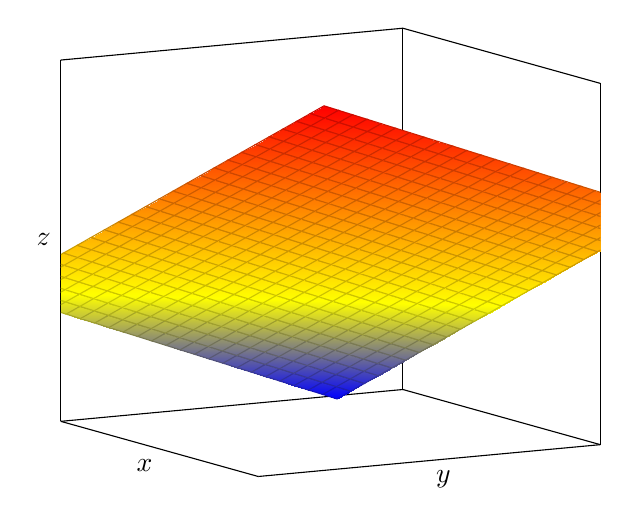
\begin{tikzpicture}
  \begin{axis}[
   view={60}{10},
   xlabel={$x$},
   ylabel={$y$},
   zlabel={$z$},
   zlabel style={rotate=90},
   xtick=\empty,
   ytick=\empty,
   ztick=\empty,
   xmin=-3,
   xmax=3,
   ymin=-5,
   ymax=5
  ]
   \addplot3[
    surf,
    colormap/hot,
    shader=faceted interp,
    ]({x}, {y}, {(2*x - y + 3) / 3});
  \end{axis}
 \end{tikzpicture}

 \caption{A \clb{plane} defined by the equation $2x - y - 3z = -3$.}
 \label{fig:plane}
\end{figure}

An \emph{underdetermined} system in three variables can contain either one or
two linear equations. In the former case, only one variable is dependent on the
other two -- we shall often call the independent variables by names such as
\emph{free variables} or \emph{parameters}. Both these names signify that a
substitution of any pair of real numbers in lieu of the two \emph{free
variables} yields a solution of the system.

For instance, the linear equation in \myref{figure}{fig:plane} is effectively a
linear system in three variables. We can choose any of the three variables to be
dependent and leave the other two free, giving thus three different descriptions
of \emph{the same} solution set. The following
equation~\eqref{eq:three-vars-one-eq} shows all of them with the chosen
dependent variable written on the left in typewriter font.
\begin{equation}
 \label{eq:three-vars-one-eq}
 \begin{array}{r l}
  \mathtt{x:} & \left\{ \left( \frac{y + 3z - 3}{2}, y, z \right) \mid y,z \in \R
  \right\}\\[1em]
  \mathtt{y:} & \left\{ \left( x, 2x - 3z + 3, z \right) \mid x,z \in \R
  \right\}\\[1em]
   \mathtt{z:} & \left\{ \left( x, y, \frac{2x - y + 3}{3} \right) \mid x,y \in
   \R \right\}
 \end{array}
\end{equation}

Linear systems in three variables and two equations are also underdetermined.
Geometrically, they correspond to arrangements of two planes in space. Those two
planes can either be parallel -- leading to the system having no solution -- or
not -- intersecting in a straight line describable as a set of triples with
exactly one free variable. In a case similar to two-dimensional linear systems,
putting the system in question into echelon form \emph{can} reveal (albeit not
always) its geometric nature.

Indeed, consider the system
\begin{equation}
 \label{eq:two-parallel-planes}
 \begin{array}{r c r c r c r}
  x & - & y & + & 2z & = & 2\\
  2x & - & 2y & + & 4z & = & 9
 \end{array}.
\end{equation}
Subtracting $\mathtt{II - 2 \cdot I}$ produces
\[
 \begin{array}{r c r c r c r}
  x & - & y & + & 2z & = & 2\\
    &   &   &   &  0 & = & 5
 \end{array},
\]
clearly a system with no solution. Subsequently, the two corresponding planes
are parallel to each other. See them depicted in
\myref{figure}{fig:two-parallel-planes}.

\begin{figure}[ht]
 \centering
 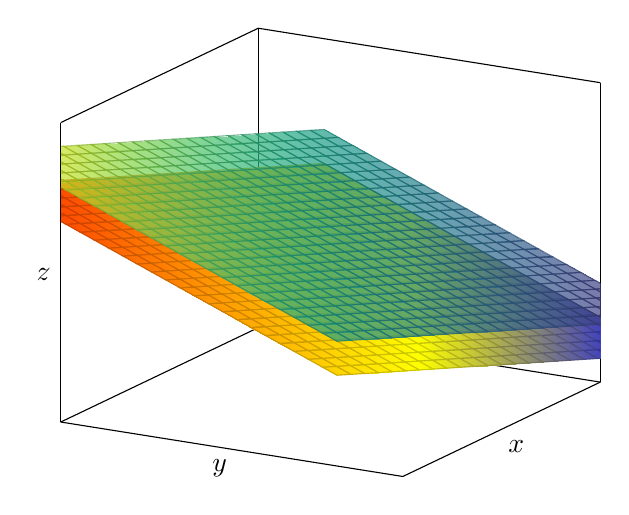
\begin{tikzpicture}
  \begin{axis}[
   view={-60}{20},
   xlabel={$x$},
   ylabel={$y$},
   zlabel={$z$},
   zlabel style={rotate=90},
   xtick=\empty,
   ytick=\empty,
   ztick=\empty,
   xmin=-3,
   xmax=3,
   ymin=-5,
   ymax=5
  ]
   \addplot3[
    surf,
    colormap/hot,
    shader=faceted interp,
   ]({x}, {y}, {(2 - x + y) / 2});
   \addplot3[
    surf,
    colormap/viridis,
    shader=faceted interp,
    opacity=0.7,
   ]({x}, {y}, {(9 - 2*x + 2*y) / 4});
  \end{axis}
 \end{tikzpicture}

 \caption{The two parallel planes from the
 system~\eqref{eq:two-parallel-planes}.}
 \label{fig:two-parallel-planes}
\end{figure}

A system of two non-parallel planes is presented below.
\begin{equation}
 \label{eq:two-non-parallel-planes}
 \begin{array}{r c r c r c r}
  x & - & y & + & 2z & = & 2\\
  2x & + & 3y & - & z & = & -1
 \end{array}
\end{equation}
By subtracting, once again, $\mathtt{II - 2 \cdot I}$, we put into the following
echelon form.
\[
 \begin{array}{r c r c r c r}
  x & - & y & + & 2z & = & 2\\
    &   & 5y & - & 5z & = & -5
 \end{array}
\]
The algorithm of Gauss-Jordan elimination limits our choice of free variables to
the ones left in the last row. We are hence to set either $y$ or $z$ loose while
caging the latter. Custom dictates to label all variables but the first of the
last row as \emph{parameters}, making $z$ the victor. The rest is just
back-substitution. We calculate $y = z - 1$ and substitute into the first
equation to receive
\[
 x - (z - 1) + 2z = 2, \quad \text{hence} \quad x = 1 - z.
\]
It follows that \emph{one possible} description of the solution set of the
system~\eqref{eq:two-non-parallel-planes} is
\[
 \left\{ (1 - z, z - 1, z) \mid z \in \R\right\}.
\]
See it depicted in \myref{figure}{fig:two-non-parallel-planes}.
\begin{figure}[ht]
 \centering
 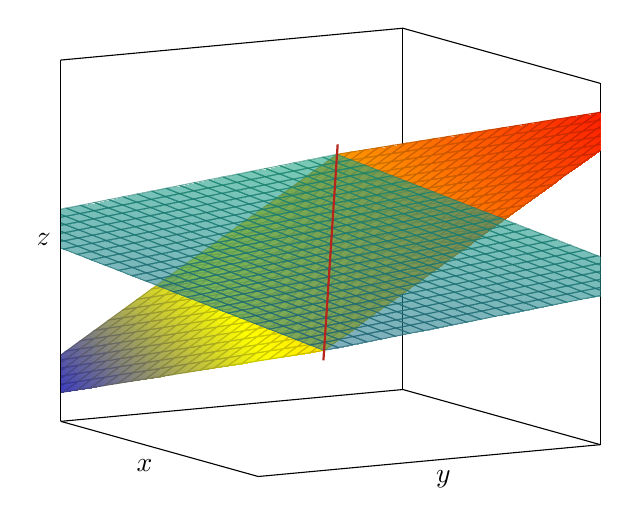
\begin{tikzpicture}
  \begin{axis}[
   view={60}{10},
   xlabel={$x$},
   ylabel={$y$},
   zlabel={$z$},
   zlabel style={rotate=90},
   xtick=\empty,
   ytick=\empty,
   ztick=\empty,
   xmin=-3,
   xmax=3,
   ymin=-5,
   ymax=5
  ]
   \addplot3[
    surf,
    colormap/hot,
    shader=faceted interp,
   ]({x}, {y}, {2*x + 3*y + 1});
   \addplot3[
    surf,
    colormap/viridis,
    shader=faceted interp,
    opacity=0.6
   ]({x}, {y}, {(2 - x + y) / 2});
  \addplot3[
   color=BrickRed,
   thick,
   smooth
  ]({x},{-x},{1-x});
  \end{axis}
 \end{tikzpicture}

 \caption{The two non-parallel planes from the
 system~\eqref{eq:two-non-parallel-planes} and their \clr{intersection}.}
 \label{fig:two-non-parallel-planes}
\end{figure}

Reaching the apex of `ideal' linear systems in three variables and three
equations, we stop to ponder the number of arrangements of three planes in
three-dimensional space. There are two obvious ones:
\begin{enumerate}
 \item All three planes are parallel to each other.
 \item Only two planes are parallel to each other.
\end{enumerate}
Corresponding to (1), resp. (2), is a linear system with two equations, resp.
one equation, with no solution.

As an example, consider the system
\begin{equation}
 \label{eq:two-parallel-one-not}
 \begin{array}{r c r c r c r}
  -x & + & 2y & - & z & = & 4\\
  x & - & 6y & + & z & = & 1\\
  x & - & 2y & + & z & = & 3
 \end{array}.
\end{equation}
Its echelon form looks like this:
\[
 \begin{array}{r c r c r c r}
  -x & + & 2y & - & z & = & 4\\
     & & -4y & & & = & 5\\
     & & & & 0 & = & 7
 \end{array}.
\]
Clearly, the third equation has no solution while the second does. This
particular system's geometrical interpretation aligns with case (2) above. It is
shown in \myref{figure}{fig:two-parallel-one-not}.
\begin{figure}[ht]
 \centering
 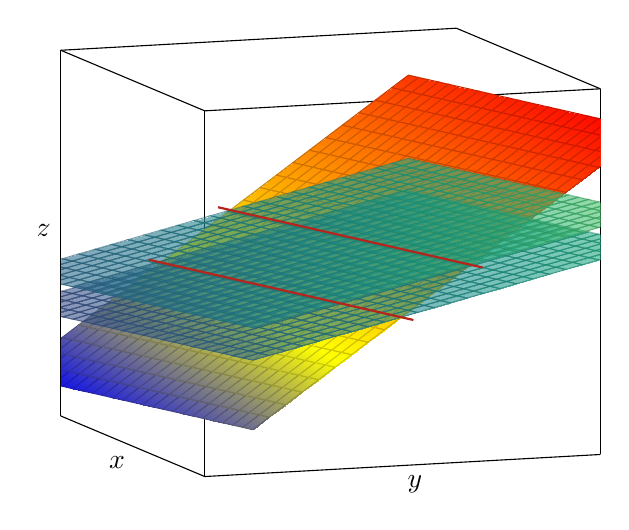
\begin{tikzpicture}
  \begin{axis}[
   view={110}{-10},
   xlabel={$x$},
   ylabel={$y$},
   zlabel={$z$},
   zlabel style={rotate=90},
   xtick=\empty,
   ytick=\empty,
   ztick=\empty,
   xmin=-3,
   xmax=3,
   ymin=-5,
   ymax=5
  ]
   \addplot3[
    surf,
    colormap/hot,
    shader=faceted interp
   ]({x}, {y}, {-x + 6*y + 1});
   \addplot3[
    surf,
    colormap/viridis,
    shader=faceted interp,
    opacity=0.6
   ]({x}, {y}, {-x + 2*y - 4});
   \addplot3[
    surf,
    colormap/viridis,
    shader=faceted interp,
    opacity=0.6
   ]({x}, {y}, {-x + 2*y + 3});
   \addplot3[
    color=BrickRed,
    thick,
    smooth
   ]({x},{1/2},{4-x});
   \addplot3[
    color=BrickRed,
    thick,
    smooth
   ]({x},{-5/4},{-x - 13/2});
  \end{axis}
 \end{tikzpicture}

 \caption{Depiction of the system~\eqref{eq:two-parallel-one-not}.}
 \label{fig:two-parallel-one-not}
\end{figure}

Finally, there are three other possible arrangements of three planes in space:
\begin{enumerate}
 \setcounter{enumi}{2}
 \item non-parallel planes that fail to have a common intersection (the
  so-often-called `tent' configuration);
 \item non-parallel planes that meet in a single point;
 \item non-parallel planes that meet in a single line.
\end{enumerate}
Of course, as always, the echelon form of a linear system can be used to
distinctively label it as any of these cases. For example, the echelon form of
the system
\begin{equation}
 \label{eq:tent}
 \begin{array}{r c r c r c r}
  x & + & 2y & - & z & = & -1\\
  2x & - & 3y & + & 2z & = & 4\\
  -x & + & 5y & - & 3z & = & 10
 \end{array}
\end{equation}
can easily be computed to be
\[
 \begin{array}{r c r c r c r}
  x & + & 2y & - & z & = & -1\\
    & & -7y & + & 4z & = & 6\\
    & & & & 0 & = & 15
 \end{array}.
\]



\section{Describing Solution Sets of Linear Systems}
\label{sec:describing-solution-sets-of-linear-systems}

In \myref{section}{sec:visualization}, we studied specific (simple) classes of
linear systems and touched upon a few important concepts, including, but not
limited to, \emph{parameters}, \emph{free variables}, \emph{underdetermined} and
\emph{overdetermined} systems.

We continue down this road and bring a general description of solution sets of
linear systems. Before we formulate the result we shall endeavour to prove in
this section, we introduce a few pieces of notation which are going to allow us
to manipulate linear systems more efficiently. Do note that behind these mere
`pieces of notation' there lies hidden a much deeper geometric meaning, to be
uncovered in later chapters.

\begin{definition}{Matrix}{matrix}
 An $m \times n$ \emph{matrix} is an array of numbers with $m$ rows and $n$
 columns. The numbers are then called \emph{entries} of the matrix.
\end{definition}

Matrices allow us to write linear systems in a much more succinct manner. For
example, the system
\[
 \begin{array}{r c r c r}
  -x & + & y & = & 2\\
  2x & - & 2y & = & 5
 \end{array}
\]
can be written using a matrix like this:
\[
 \left(
  \begin{matrix*}[r]
   -1 & 1\\
   2 & -2
  \end{matrix*}
  \hspace{1mm}
 \right|
 \left.
  \begin{matrix*}[r]
   2\\
   5
  \end{matrix*}
 \right),
\]
abusing the fact that the same variables are located in a single column and each
row is a single linear equation. The bar on the right side simply serves to
divide left sides of the equations from right ones.

Matrices make Gauss-Jordan elimination easier to perform and keep track of its
progress. The matrix of the eliminated system looks like this
\[
 \left(
  \begin{matrix*}[r]
   -1 & 1\\
   0 & 0
  \end{matrix*}
  \hspace{1mm}
 \right|
 \left.
  \begin{matrix*}[r]
   2\\
   9
  \end{matrix*}
 \right)
\]
and has been reached by the row operation $\mathtt{II + 2I}$.

Certain matrices are special (for reasons soon to be revealed) and we call them
\emph{vectors}.

\begin{definition}{Vector}{vector}
 A \emph{column vector} is an $n \times 1$ matrix (that is, matrix with a single
 column) and a \emph{row vector} is a $1 \times n$ matrix (a matrix with a
 single row). As column vectors are the `default', we call them simply
 \emph{vectors}.
\end{definition}

There exists an obvious bijection between tuples $(v_1,\ldots,v_n)$ and column
vectors $\mathbf{v} = \begin{psmallmatrix} v_1\\[-4pt]\vdots\\v_n
\end{psmallmatrix}$. Consequently, we say that a vector $\mathbf{v}$ with
entries $v_1,\ldots,v_n$ \emph{solves} a linear equation
\[
 a_1x_1 + a_2x_2 + \ldots + a_nx_n = c
\]
if the tuple $(v_1,\ldots,v_n)$ does.

The addition of vectors and their multiplication by a number are defined
naturally.

\begin{definition}{Adding vectors}{adding-vectors}
 Given vectors
 \[
  \mathbf{u} =
  \begin{pmatrix}
   u_1\\
   u_2\\
   \vdots\\
   u_n
  \end{pmatrix}
  \quad \text{and} \quad 
  \mathbf{v} = 
  \begin{pmatrix}
   v_1\\
   v_2\\
   \vdots\\
   v_n
  \end{pmatrix},
 \]
 their \emph{sum} is defined as the vector
 \[
  \mathbf{u} + \mathbf{v} \coloneqq 
  \begin{pmatrix}
   u_1 + v_1\\
   u_2 + v_2\\
   \vdots\\
   u_n + v_n
  \end{pmatrix}.
 \]
\end{definition}

\begin{definition}{Multiplying vector by a number}{multiplying-vector-by-a-number}
 Given a vector
 \[
  \mathbf{v} = 
  \begin{pmatrix}
   v_1\\
   v_2\\
   \vdots\\
   v_n
  \end{pmatrix}
 \]
 and a number $c$, the \emph{scalar $c$-multiple of $\mathbf{v}$} is the vector
 \[
  c \mathbf{v} \coloneqq 
  \begin{pmatrix}
   cv_1\\
   cv_2\\
   \vdots\\
   cv_n
  \end{pmatrix}.
 \]
 The multiplying number $c$ is often referred to as a \emph{scalar}.
\end{definition}

We further need to discuss the concept of \emph{free variables} and
\emph{parameters}.

In the \hyperref[sec:visualization]{previous section}, we described the solution
set of the system~\eqref{eq:two-vars-one-eq} using three different ways. In each
case, two of the variables were independent and the third was their linear
combination. We style the two independent variables, \emph{parameters}. Vaguely
said, a \emph{parameter} is a variable on the value thereof other variables
depend. 

We're now equipped to formulate a result about the `shape' of a linear system's
solution set with a rather far-reaching importance.

\begin{theorem}{Solution set of a linear system}{solution-set-of-a-linear-system}
 The solution set of every linear system can be written in the form
 \[
  \{\mathbf{u} + t_1 \mathbf{v_1} + t_2 \mathbf{v_2} + \ldots +
  t_n\mathbf{v_n}\},
 \]
 where $\mathbf{u}$ is a particular solution, $\mathbf{v_1},\ldots,\mathbf{v_n}$
 are vectors.
\end{theorem}

\section{Applications}
\label{sec:applications}

In this final section of \myref{chapter}{chap:linear-systems}, we focus on some
`real-world' applications of linear systems and, more generally, on methods of
solving linear systems using computers.

The software we shall employ toward this end styles
\href{https://www.sagemath.org/}{SageMath}. It's a free open-source mathematics
software capable of numeric and symbolic manipulation of objects from various
fields of mathematics, linear algebra included. It can be installed on most
operating systems following the
\href{https://doc.sagemath.org/html/en/installation/index.html}{official guide}.

SageMath is essentially a terminal-based software and out of the box offers no
graphical user interface. Upon launch, 

